\documentclass{article}
\usepackage{amsmath}
\usepackage{amssymb}
\usepackage{graphicx}
\usepackage{hyperref}
\usepackage[version=4]{mhchem}

\title{Problem 6}
\date{}

\begin{document}
\maketitle

\section*{Problem}
As shown in the figure below, in \(\triangle A B C, \angle A B D=2 \angle C . A D\) is the angle bisector of \(\angle A . B D \perp A D\) at \(D\). Show that \(B D\) \(=\frac{1}{2}(A C-A B)\).\\
\centering
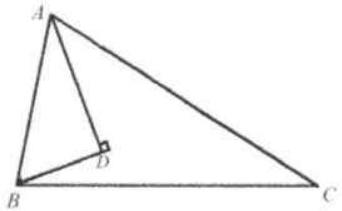
\includegraphics[width=\textwidth]{images/problem_image_1.jpg}

\section*{Solution}
Extend \(B D\) to meet \(A C\) at \(M\).\\
Since \(A D\) is the angle bisector of \(\angle A\). and \(B D \perp A D\), \(\angle B A D=\angle M A D=\alpha, A B=A M, \angle A B D=\angle A M D=\beta\).\\
Since \(\angle A B D=\angle A M D=2 \angle C, \angle M C B=\angle M B C=\gamma\) \(A M=2 B D=M C=A C-A M \Rightarrow B D=\frac{1}{2}(A C-A B)\).\\
\centering
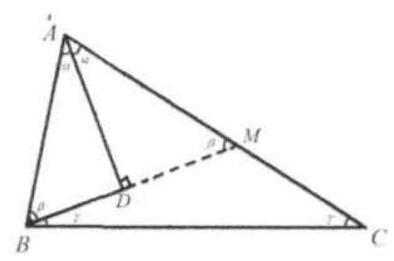
\includegraphics[width=\textwidth]{images/reasoning_image_1.jpg}

\end{document}
